%%% AFUP Lyon 2012
%%%
%%% Pour beaucoup de développeurs le SQL se limite au travail d’un ORM ou
%%% bien à ces chaînes de caractères qu’il faut embarquer dans le code, de
%%% manière plus ou moins statiques, et dont on aimerait bien se passer…
%%%
%%% Nous allons voir en quelques exemples pratique comment faire SQL votre
%%% meilleur outil dès que vous avez besoin d’analyser des données.

\documentclass{beamer}

\usepackage{beamerthemesplit}
\usepackage[utf8]{inputenc}
%% \usetheme{AnnArbor}
\usetheme{Boadilla}
%% \usetheme{Pittsburgh}
%% \usecolortheme{beaver}
\beamertemplatetransparentcovered

\title{PostgreSQL}
\subtitle{quand on est développeur}
\author{Dimitri Fontaine \texttt{dimitri@2ndQuadrant.fr}}
\date{31 Octobre 2012}
\logo{
\includegraphics[height=0.4cm]{2ndQuadrant-cross.png}}

\begin{document}

\frame{\titlepage}

\section{Introduction}

\begin{frame}[fragile]
  \frametitle{Dimitri Fontaine}

  \begin{center}
    \textbf{2ndQuadrant France}
    \linebreak
    PostgreSQL Major Contributor
  \end{center}
  \linebreak

\begin{columns}[c]
\column{.75\textwidth} 

  \begin{itemize}
   \item<2-> \texttt{pgloader}, \texttt{prefix}, \texttt{skytools}, \texttt{debian}, …
   \item<2-> \texttt{\textbf{CREATE EXTENSION}}
   \item<3-> \texttt{\textbf{CREATE EVENT TRIGGER}}
   \item<3-> \textit{Bi-Directional Réplication}
   \item<4-> \textit{Partitionnement}
  \end{itemize}  

\column{.25\textwidth}
\begin{center}
  
\includegraphics[height=5em]{bulle-blue-icon.png}
\end{center}
\end{columns}
\end{frame}

\begin{frame}[fragile]
  \frametitle{Outils et languages de développement}

  \center{PHP est une petite partie de votre métier de développeur web.}

\begin{columns}[c]
\column{.3\textwidth} 

  \begin{itemize}
   \item HTML
   \item Javascript
   \item \textit{JQuery}
   \item \alert{SQL}
  \end{itemize}  

\column{.7\textwidth}
  \begin{center}
    
\includegraphics[height=13em]{skill-set.jpg}
  \end{center}
\end{columns}
\end{frame}

\section{Projet}

\frame{
  \frametitle{Définition d'un projet simple}

\begin{center}
  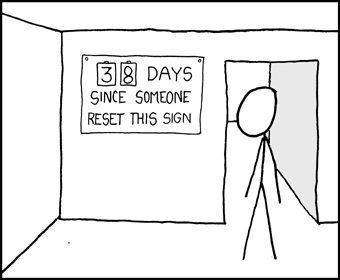
\includegraphics[height=2.3in]{reset.png}
\end{center}    
}

\begin{frame}[fragile]
  \frametitle{Définition du projet}

  Nous allons avancer à partir d'un exemple

  \begin{itemize}
    \item<1-> Gestion d'un compteur avec cycles
    \item<2-> Ajout de nouvelles mesures dans le temps
    \item<3-> Consolidation mensuelle pour facturation
    \item<4-> Analyze du comportement du compteur
  \end{itemize}
\end{frame}

\begin{frame}[fragile]
  \frametitle{SQL commence avec les DDLs}

  \center{\textbf{\textit{Joe Celko}}: \texttt{80\%} du boulot est dans les DDL}
  \linebreak

\begin{example}[DDL]
\begin{verbatim}
create table mesures(date timestamptz primary key,
                     mesure integer);

dim=# \d mesures
\d mesures
            Table "public.mesures"
 Column |           Type           | Modifiers 
--------+--------------------------+-----------
 date   | timestamp with time zone | not null
 mesure | integer                  | 
Indexes:
    "mesures_pkey" PRIMARY KEY, btree (date)
\end{verbatim}
\end{example}
\end{frame}

\begin{frame}[fragile]
  \frametitle{Simplifions pour la présentation}

\begin{verbatim}
create table measures(tick int, nb int);

insert into measures
     values (1, 0), (2, 10), (3, 20), (4, 30), (5, 40),
            (6, 0), (7, 20), (8, 30), (9, 60);
\end{verbatim}
\end{frame}

\begin{frame}[fragile]
  \frametitle{Les données de test}

  Mesures issues de notre compteur, avec un démarrage à 0 et un
  \textit{reset} en milieu de cycle. La consommation globale est ici
  \alert{\texttt{40 + 60 = 100}}.

\begin{verbatim}
select * from measures;
 tick | nb 
------+----
    1 |  0
    2 | 10
    3 | 20
    4 | 30
    5 | 40
    6 |  0
    7 | 20
    8 | 30
    9 | 60
(9 rows)
\end{verbatim}
\end{frame}

\begin{frame}[fragile]
  \frametitle{PostgreSQL sait travailler avec des tableaux}

\begin{verbatim}
select array_agg(nb) from measures;
         array_agg          
----------------------------
 {0,10,20,30,40,0,20,30,60}
(1 row)
\end{verbatim}
\end{frame}

\begin{frame}[fragile]
  \frametitle{Trouver les points avant reset}

\begin{columns}
\column{.65\textwidth}
\center{\textit{Écrire une requête \alert{SQL} ici}}
\column{.35\textwidth}
\begin{verbatim}
 tick | nb | max 
------+----+-----
    1 |  0 |    
    2 | 10 |    
    3 | 20 |    
    4 | 30 |    
    5 | 40 |  40
    6 |  0 |    
    7 | 20 |    
    8 | 30 |    
    9 | 60 |  60
(9 rows)
\end{verbatim}
\end{columns}
\end{frame}

\begin{frame}[fragile]
  \frametitle{Window Functions: \texttt{lead() over()}}

\begin{columns}
\column{.65\textwidth}
\begin{verbatim}
  select tick,
         nb,
         lead(nb) over (order by tick)
    from measures;
\end{verbatim}

\column{.35\textwidth}
\begin{verbatim}
 tick | nb | lead 
------+----+------
    1 |  0 |   10
    2 | 10 |   20
    3 | 20 |   30
    4 | 30 |   40
    5 | 40 |    0
    6 |  0 |   20
    7 | 20 |   30
    8 | 30 |   60
    9 | 60 |     
(9 rows)
\end{verbatim}
\end{columns}
\end{frame}

\begin{frame}[fragile]
  \frametitle{Window Functions et \texttt{CASE}}

\begin{columns}
\column{.65\textwidth}
\begin{verbatim}
  select tick, nb,
         case when lead(nb) over w < nb
              then nb

              when lead(nb) over w is null
              then nb

              else null
          end as max
    from measures
  window w as (order by tick);
\end{verbatim}
\column{.35\textwidth}
\begin{verbatim}
 tick | nb | max 
------+----+-----
    1 |  0 |    
    2 | 10 |    
    3 | 20 |    
    4 | 30 |    
    5 | 40 |  40
    6 |  0 |    
    7 | 20 |    
    8 | 30 |    
    9 | 60 |  60
(9 rows)
\end{verbatim}
\end{columns}
\end{frame}

\begin{frame}[fragile]
  \frametitle{Window Functions et clause \texttt{WHERE}}

\begin{verbatim}
with t(tick, nb, max) as (
  select tick, nb,
         case when lead(nb) over w < nb then nb
              when lead(nb) over w is null then nb
              else null
          end as max
    from measures
  window w as (order by tick)
)
select tick, nb, max from t where max is not null;
 tick | nb | max 
------+----+-----
    5 | 40 |  40
    9 | 60 |  60
(2 rows)
\end{verbatim}
\end{frame}

\begin{frame}[fragile]
  \frametitle{Common Table Expressions avec \texttt{WITH}}

\begin{verbatim}
with t(tops) as (
  select case when lead(nb) over w < nb then nb
              when lead(nb) over w is null then nb
              else null
          end as max
    from measures
  window w as (order by tick)
)
select sum(tops) from t;
 sum 
-----
 100
(1 row)
\end{verbatim}
\end{frame}

\frame{
  \frametitle{Consomation Globale: problème résolu, SQL, 9 lignes}

  \begin{center}
    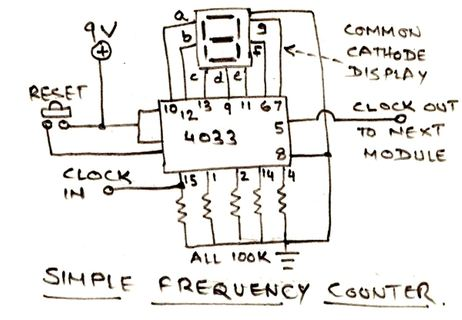
\includegraphics[height=2.3in]{reset-circuit-thumbnail.jpg}
  \end{center}
}

\begin{frame}[fragile]
  \frametitle{Création de plusieurs cycles}

\begin{verbatim}
insert into measures
     values (10, 0), (11, 10), (12, 30), (13, 35), (14, 45),
            (15, 25), (16, 50), (17, 100), (18, 110);
\end{verbatim}
\end{frame}

\begin{frame}[fragile]
  \frametitle{Visualisation de plusieurs cycles}

\begin{verbatim}
with t(tick, nb, max) as (
  select tick, nb,
         case when lead(nb) over w < nb then nb
              when lead(nb) over w is null then nb
              else null
          end as max
    from measures
  window w as (order by tick)
)
select tick, nb, max from t where max is not null;
 tick | nb  | max 
------+-----+-----
    5 |  40 |  40
    9 |  60 |  60
   14 |  45 |  45
   18 | 110 | 110
(4 rows)
\end{verbatim}
\end{frame}


\begin{frame}[fragile]
  \frametitle{Consommation globale avec plusieurs cycles}

\begin{verbatim}
with t(tops) as (
  select case when lead(nb) over w < nb then nb
              when lead(nb) over w is null then nb
              else null
          end as max
    from measures
  window w as (order by tick)
)
select sum(tops) from t;
 sum 
-----
 255
(1 row)
\end{verbatim}
\end{frame}

\begin{frame}[fragile]
  \frametitle{Limiter la période de mesures}

  \begin{center}
    
\includegraphics[height=2.3in]{calendar.png}
  \end{center}
\end{frame}

\begin{frame}[fragile]
  \frametitle{Limiter la période de mesures}

\begin{columns}
\column{.65\textwidth}
\begin{verbatim}
select tick, nb
  from measures
 where tick >= 4 and tick < 14;
\end{verbatim}

\column{.35\textwidth}
\begin{verbatim}
 tick | nb 
------+----
    4 | 30
    5 | 40
    6 |  0
    7 | 20
    8 | 30
    9 | 60
   10 |  0
   11 | 10
   12 | 30
   13 | 35
\end{verbatim}
\end{columns}
\end{frame}

\begin{frame}[fragile]
  \frametitle{Limiter la période de mesures, \texttt{first\_value}}

\begin{columns}
\column{.65\textwidth}
\begin{verbatim}
  select nb,
     first_value(nb) over w as first,
     case when lead(nb) over w < nb
          then nb

          when lead(nb) over w is null
          then nb

          else null
      end as max
    from measures
   where tick >= 4 and tick < 14
  window w as (order by tick);
\end{verbatim}

\column{.35\textwidth}
\begin{verbatim}
 nb | first | max 
----+-------+-----
 30 |    30 |    
 40 |    30 |  40
  0 |    30 |    
 20 |    30 |    
 30 |    30 |    
 60 |    30 |  60
  0 |    30 |    
 10 |    30 |    
 30 |    30 |    
 35 |    30 |  35
(10 rows)
\end{verbatim}
\end{columns}
\end{frame}

\begin{frame}[fragile]
  \frametitle{Consommation globale dans une période limitée}

\begin{verbatim}
with t as (
  select tick,
         first_value(nb) over w as first,
         case when lead(nb) over w < nb then nb
              when lead(nb) over w is null then nb
              else null
          end as max
    from measures
   where tick >= 4 and tick < 14
  window w as (order by tick)
)
select sum(max) - min(first) as sum from t;
 sum 
-----
 105
(1 row)
\end{verbatim}
\end{frame}

\begin{frame}[fragile]
  \frametitle{Comportement du \textit{reset} du compteur}

  \begin{center}
    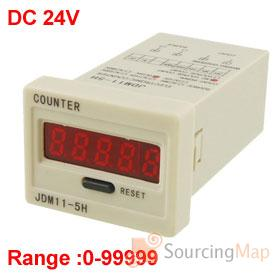
\includegraphics[height=2.3in]{reset-elect.jpg}
  \end{center}
  
\end{frame}

\begin{frame}[fragile]
  \frametitle{Partitionnement par \textit{reset}}

\begin{verbatim}
with tops as (
  select tick, nb,
         case when lead(nb) over w < nb then nb
              when lead(nb) over w is null then nb
             else null
         end as max
    from measures
  window w as (order by tick)
)
  select tick, nb, max,
         (select tick
            from tops t2
           where t2.tick >= t1.tick and max is not null
        order by t2.tick
           limit 1) as p
    from tops t1;
\end{verbatim}
\end{frame}

\begin{frame}[fragile]
  \frametitle{Partitionnement par \textit{reset}}

\begin{columns}
\column{.5\textwidth}
\begin{verbatim}
 tick | nb  | max | p  
------+-----+-----+----
    1 |   0 |     |  5
    2 |  10 |     |  5
    3 |  20 |     |  5
    4 |  30 |     |  5
    5 |  40 |  40 |  5
    6 |   0 |     |  9
    7 |  20 |     |  9
    8 |  30 |     |  9
    9 |  60 |  60 |  9
\end{verbatim}

\column{.5\textwidth}
\begin{verbatim}
 tick | nb  | max | p  
------+-----+-----+----
   10 |   0 |     | 14
   11 |  10 |     | 14
   12 |  30 |     | 14
   13 |  35 |     | 14
   14 |  45 |  45 | 14
   15 |  25 |     | 18
   16 |  50 |     | 18
   17 | 100 |     | 18
   18 | 110 | 110 | 18
\end{verbatim}
\end{columns}
\end{frame}

\begin{frame}[fragile]
  \frametitle{Consommation globale par range avec \texttt{PARTITION BY}}

\begin{columns}
\column{.65\textwidth}
\begin{verbatim}
with tops as ( <case lead() over()> ),
     parts as ( <self join limit 1> ),
     ranges as (
  select
      first_value(tick) over w as start,
      last_value(tick) over w as end,
      max(max) over w
    from parts
  window w as (partition by p
               order by tick)
)
select * from ranges
 where max is not null;
\end{verbatim}

\column{.35\textwidth}
\begin{verbatim}
 start | end | max 
-------+-----+-----
     1 |   5 |  40
     6 |   9 |  60
    10 |  14 |  45
    15 |  18 | 110
(4 rows)
\end{verbatim}
\end{columns}
\end{frame}

\begin{frame}[fragile]
  \frametitle{Consommation globale par range avec \texttt{in4range()}}

\begin{columns}
\column{.65\textwidth}
\begin{verbatim}
with tops as ( <case lead() over()> ),
     parts as ( <self join limit 1> ),
     ranges as (
  select int4range(
           first_value(tick) over w,
           last_value(tick) over w,
           '[]') as range,
         max(max) over w as compteur
    from parts
  window w as (partition by p
               order by tick)
)
select range, compteur
  from ranges
 where compteur is not null;
\end{verbatim}
\column{.35\textwidth}
\begin{verbatim}
  range  | compteur 
---------+----------
 [1,6)   |       40
 [6,10)  |       60
 [10,15) |       45
 [15,19) |      110
(4 rows)
\end{verbatim}
\end{columns}
\end{frame}

\begin{frame}[fragile]
  \frametitle{Consommation globale par range avec \texttt{@>}}

\begin{columns}
\column{.65\textwidth}
\begin{verbatim}
with tops as ( <case lead() over()> ),
     parts as ( <self join limit 1> ),
     ranges as ( <int4range()
                  over (partition by
                        order by)> )
select range, compteur
  from ranges
 where compteur is not null
       and range @> 11;
\end{verbatim}

\column{.35\textwidth}
\begin{verbatim}
  range  | compteur 
---------+----------
 [10,15) |       45
(1 row)
\end{verbatim}
\end{columns}
\end{frame}


\section{Conclusion}

\frame{
  \frametitle{Conclusion}

\begin{center}
  SQL fait partie de vos outils de développeur, tirez-en le meilleur!
  \linebreak
  \linebreak

  \begin{center}
    
\includegraphics[height=2.1in]{skill-set.jpg}
  \end{center}
\end{center}
}

\end{document}
